% !TEX encoding = UTF-8 Unicode
\documentclass[a4paper, 11pt]{report}

\usepackage[margin=3cm]{geometry}
\usepackage{ifxetex}

\ifxetex
  \usepackage{fontspec}
\else
  \usepackage[utf8]{inputenc}
  \usepackage[T1]{fontenc}
  \usepackage{lmodern} % Improve vectorial font
\fi

\usepackage{graphicx} % Required for includegraphics

\usepackage{url, hyperref} % Useful to make links clickable amongst others

\usepackage{float} % Put figures where you actually want [H]

\usepackage{tikz} % Beautiful drawings
\usetikzlibrary{arrows}

\usepackage{amssymb}

\usepackage[linesnumbered, ruled, french,onelanguage]{algorithm2e}
\makeatletter
\g@addto@macro{\@algocf@init}{\SetKwInput{KwOut}{Sortie}}
\makeatother

% Fancyhdr (headers and footers)
% ==============================
\usepackage{lastpage}
\usepackage{fancyhdr}
\pagestyle{fancy}
\cfoot{\thepage~sur \pageref{LastPage}} % style de numéro de page
% - Fancypagestyle 'plain' pour les pages de chapitres -
\fancypagestyle{plain}{%
\fancyhf{} % vide l’en-tête et le pied~de~page.
\fancyfoot[C]{\thepage~sur \pageref{LastPage}} % style de numéro de page
\renewcommand{\headrulewidth}{0pt}
\renewcommand{\footrulewidth}{0pt}}
% - Chapter mark -
\renewcommand{\chaptermark}[1]{%
\markboth{\MakeUppercase{%
\chaptername}\ \thechapter.%
\ #1}{}}
% - Section mark -
\renewcommand{\sectionmark}[1]{\markright{\thesection.\ #1}}
% ==============================

% Title page elements declarations
% ================================================================

% UNICAEN Logo
% ------------
\definecolor{logo}{rgb}{0,0,0} % Background colour of the logo

\tikzset{ligne/.style={line width=5pt, color=white},
         cover/.style={line width=5pt, color=logo}}

\newcommand{\unicaen}{%
\begin{tikzpicture}
% Big black circle:
\fill [fill=logo] (-0.2,0) circle (4);
% Letter U:
\draw[ligne] (-3,0.52) -- ++(0,-0.83); % Left bar of the U
\coordinate (baseu) at (-3,-0.25);
\draw[ligne] (baseu) .. controls +(0,-0.4) and +(-0.1,-0.4) .. (-2.2,-0.28);
% Letter N:
\draw[ligne] (-2.2,-0.35) -- ++(0,0.70) -- ++(-45:0.98)
                                                            -- ++(90:0.85);
\draw[cover] (-2.2,-0.52) ++(0,0.87) ++(0:-6.2pt) -- ++(-45:1.4); % Cover
\draw[cover] (-1.51,0.27) node{\footnotesize$\blacksquare$}; % Cover

% Letter C:
\draw[ligne] (0.1,1.2) arc (90:270:1.2);
\draw[cover] (-1.1,0) node{\footnotesize$\blacksquare$}; % Cover
% Letter A (triangle):
\coordinate (triangletop) at (0,0.4);
\draw [ligne] (triangletop) -- ++(60:-1) -- ++(1,0)
                                                  -- ++(-60:-1) -- cycle;
\draw[cover] (triangletop) ++(0:-5pt) -- ++(-60:1.2); % Cover
% Letter E:
\draw[ligne] (0.8,0.45) -- ++(0.8,0);
\draw[ligne] (0.8,0) -- ++(0.8,0);
\draw[ligne] (0.8,-0.45) -- ++(0.8,0);
% Letter N:
\draw[ligne] (2,-0.52) -- ++(0,0.87) -- ++(-45:0.98)
                                                            -- ++(90:0.85);
\draw[cover] (2,-0.52) ++(0,0.87) ++(0:-6pt) -- ++(-45:1.4); % Cover
\end{tikzpicture}}

% New elements
% ----------------------
\makeatletter
\def\@university{}
\newcommand{\university}[1]{\def\@university{#1}}
%
\def\@department{}
\newcommand{\department}[1]{\def\@department{#1}}
%
\def\@subject{}
\newcommand{\subject}[1]{\def\@subject{#1}}
\makeatother

% ----- Title page customisation -----
\makeatletter
\newcommand{\mytitle}{
  \begin{titlepage} % Create the command to include the title page in the document
  \hbox{
    \parbox[b]{.4\textwidth}{ % Paragraph box which restricts text to less than the width of the page
      \resizebox{.3\textwidth}{!}{\unicaen}\\[1em]
      {\noindent\LARGE\textsc\@university}\\[1em] % University
      {\noindent\@department} % Department
      \vskip.65\textheight % Skip from the bottom of the page to the text (\parbox[b])
    }
    %\hspace*{.2\textwidth} % Space to the left of the title page
    \rule{1pt}{\textheight} % Vertical line
    \hspace*{0.05\textwidth} % Space between the vertical line and title page text
    \parbox[b]{0.75\textwidth}{
      {\noindent\Huge\bfseries\@title} % Title
      \vskip 5em%
      {\large\textit{\@subject}} % Subject
      \vskip 9em%
      \@author % Author(s) name(s)
      \vskip 0.4\textheight % Skip between the title block and the publisher
      {\noindent\@date}\\[\baselineskip] % Date
    }
  }
  \end{titlepage}
}
\makeatother
% ============================================================
% end of title page declarations

\usepackage[french]{babel} % language package

\title{Sokoban}
\date{\today}
\author{Maël Querré\\
        Alexis Mortelier\\
        Vincent De Menezes\\
        Christina Williamson}
\university{Université\\[.3em]
            Caen\\[.3em]
            Normandie}
\department{Département d'informatique}
\subject{Travail Personnel Approfondi}

\begin{document}

\mytitle

\tableofcontents


\chapter{Objectifs du projet}

\section{Description du concept}

\emph{Sokoban} est un jeu vidéo de puzzle inventé au Japon.

\subsection{Règles du jeu \cite{wiki:Sokoban}}

Gardien d'entrepôt (divisé en cases carrées), le joueur doit ranger des caisses sur des cases cibles. Il peut se déplacer dans les quatre directions, et pousser (mais pas tirer) une seule caisse à la fois. Une fois toutes les caisses rangées (c'est parfois un vrai casse-tête), le niveau est réussi et le joueur passe au niveau suivant, plus difficile en général. L'idéal est de réussir avec le moins de coups possibles (déplacements et poussées).

\section{Ce qu'il fallait faire}

Dans un premier temps, il s'agit de réaliser un jeu jouable pour un humain avec importation de niveaux. Pour cela, des formats de données (comme .xsb, .sok ou .stb) dédiés peuvent être utilisés. Une interface graphique devra également être réalisée. Une fois ce travail préliminaire fini, il conviendra de proposer une fonctionnalité de résolution automatique de niveau (comme l'algorithme A*) et de permettre de faire jouer humain et ordinateur en parallèle. Enfin, une dernière étape consiste à rendre \emph{anytime} l'algorithme de l'intelligence artificielle : cette dernière est obligée de jouer dès que l'humain fait un mouvement.

\section{Ce qui existe déjà}

Pour l'intelligence artificielle nous aurons besoin de calculer si le jeu est bloqué à chaque déplacement. Le Sokoban YASC ajoute aux fonctionnalités du Sokoban la possibilité de faire des retours en arrière mais surtout permettre d'éviter les situations où le jeu se retrouve bloqué.

\chapter{Fonctionnalités implémentées}

\section{Description des fonctionnalités}

\subsection{Réalisation du jeu}
Le jeu du Sokoban est un casse tête se jouant sur une grille. Chaque case de la grille possède un type d'élément, il en existe 6 :
\begin{itemize}
    \item type vide
    \item type mur
    \item type caisse
    \item type joueur
    \item type cible
    \item type caisse sur cible
    \item type joueur sur cible
\end{itemize}
Pour modéliser ce problème nous avons décidé de séparer le jeu en 3 parties (plateau, élément du plateau, chargement des niveaux).

\subsubsection{Plateau}
Afin de générer un plateau nous avons eu l'idée de créer un tableau possédant les éléments du plateau. Dans cette classe nous établissons toute les règles nécessaires pour le fonctionnement du Sokoban. L'initialisation de la partie se fait par cette classe comme les méthodes de déplacements et 
Cette classe permet d'initialiser une partie et d'établir les déplacements sur le plateau, elle nous permet de detecter si la partie est finie.
Il est nécessaire de lui fournir des informations afin qu'elle puisse simuler une partie, pour cela elle utilise la classe de chargement des niveaux pour obtenir les informations nécessaires pour lancer la partie.

\subsubsection{Element du plateau}
Les elements du plateau vont correspondre à nos types d'états, la classe va initialiser les 6 états vu précedemment. Elle a besoin de methodes de restitution afin qu'elle puisse communiquer avec le plateau. En effet, le plateau va interroger le type de la case lorsqu'on voudra agir sur celle-ci. Elle possède aussi une méthode permettant de changer son état, ce qui servira pour les déplacements demandés.\\

Cette classe va être aussi utilisé par la classe d'Intelligence Artificielle (voir \pageref{IA}). Celle-ci aura besoin d'autres informations que les types des cases afin que celle-ci puisse se reperer sur le plateau. Cette classe doit restituer trois couches :
\begin{itemize}
    \item couche de vérification
    \item couche de trajectoire
    \item couche de deadlock \pageref{deadlock}
\end{itemize}

\vskip 1em

La couche de vérification permet de vérifier chaque case du plateau en considérant le pi corral (page~\pageref{corral}). La détection de pi corral nous permet de gagner du temps d'efficacité lors de la recherche dans les trois couches. Cette couche doit être réinitialisée à chaque utilisation de celle-ci, car, elle sert pour la détection de destination de caisse mais aussi lors du calcul des couches de trajectoires et de deadlock. Remarque : cette couche sert d'initialisation pour tous les autres calculs de l'intelligence artificielle.\\

La couche de trajectoire va attribuer à la case ciblé un nombre. Ce nombre permet de connaître le nombre de case entre la position d'origine et la case ciblé. Remarque : en utilisant une décrementation pour détecter la case voisine nous pouvons déduire le meilleur chemin entre la case ciblé et l'origine.\\

La couche de deadlock est une couche booléenne, elle permet de savoir si la case ciblé est une case gelée \pageref{gele}.

\subsubsection{Chargement des niveaux}
Le chargement des niveaux est une classe permettant d'obtenir a partir d'un fichier les informations nécessaires lors de la création d'un plateau. Elle doit donc restituer une liste de chaine de caractère afin que la classe plateau puisse initialiser le niveau. La classe possède deux méthodes, sauvegarde et chargement de niveau permettant à l'utilisateur de sauvegarder sa progression. Pour le fonctionnement de la classe plateau, cette classe doit pouvoir indiquer la largeur et la hauteur de la grille. Une méthode existe donc permettant d'obtenir toutes les informations nécessaire à l'initialisation d'un niveau.\\ \\

Cette conceptualisation du jeu nous permet de faciliter l'acces aux informations pour l'intelligence artificielle mais aussi facilité la communication avec l'interface graphique. Lors du projet nous avons eu une nouvelle méthode d'approche afin de résoudre le probleme donné, celle-ci oublie le principe de tableau d'element du plateau. Elle est composée d'ensemble. Ces ensembles représente trois parmis six des types présentés, il y a donc un ensemble pour les caisses, les destinations et le curseur. Cette méthode est très efficace pour le déplacement via la superposition des types (une caisse sur une destination deviens un nouveau type dans l'univers du sokoban alors qu'avec cette méthode il y a juste les mêmes positions dans deux ensembles, caisse et destination). Mais cette méthode ne permet pas de simuler nos trois couches ce qui rends la vision de l'intelligence artificielle sur le plateau difficile, bien qu'avec cette nouvelle méthode d'autres problèmes peuvent être éviter.

\subsection{Modélisation de l'intelligence artificielle}

\label{IA}


Avant de pouvoir faire fonctionner notre intelligence artificielle, il faut lui imposer des limites. Les limites seront calculées dans un premier temps par les \emph{deadlocks}\footnote{voir chapitre~\ref{deadlock}}.

D'autres limites peuvent être ajoutées comme la vérification d'un plateau déjà effectué ou bien une simple vérification de direction afin d'éviter que l'intelligence artificielle ne calcule trop de coups avant de s'apercevoir qu'elle aurait pu obtenir une meilleure situation à l'aide d'un guidage de direction.

L'intelligence artificielle ignore la notion de \emph{deadlock}, pour cela il faut lui faire détecter les situations de \emph{deadlocks} à l'aide de fonctions. Dans un premier temps, il est facile de détecter un simple \emph{deadlock}, il suffit de partir des destinations puis de tirer une caisse sur toutes les caisses possibles du plateau. Une fois ce processus fini, toutes les cases qui n'ont pas été visitées par la caisse sont automatiquement des cases gelées\footnote{voir chapitre~\ref{gele}}. Pour détecter les impasses, le principe est assez simple. Nous détectons l'entrée d'un tunnel et nous vérifions que pour toutes les cases du tunnel, il n'y ait pas d'obstacle comme un mur ou une caisse (en effet, il préférable de détecter aussi les cases gelées dans le tunnel, car un tunnel qui effectue un virage n'est pas reconnu comme impasse pour la mobilité du joueur mais ne pourra pas faire passer une caisse).

À chaque déplacement d'une caisse, nous vérifions si la caisse ne se trouve pas sur une situation de deadlock à l'aide d'un algorithme qui va détecter si une case est gelée sur un axe :

\begin{algorithm}
\KwIn{Des positions $i$ et $j$ correspondant à une coordonnée d'une case à vérifier}
\KwOut{Une valeur booléenne correspondant à l'axe bloqué}
$haut \gets false$\;
$bas \gets false$\;
\uIf{la case en haut et en bas n'est pas un mur}{
	\uIf{la case en haut ou en bas n'est pas une case gelée}{
		\uIf{la case en haut est une caisse}{
			$haut \gets true$\;
		}
		\uIf{la case en bas est une caisse}{
			$bas \gets true$\;
		}
		\uIf{$haut == false$ et $bas == false$}{
			\Return{false}\;
		}
	}
}
\Return{true}\;
\caption{Détection d'une situation de deadlock sur l'axe horizontal}
\end{algorithm}

Pour savoir si notre case est une case gelée, nous lui attribuons une \og couche \fg{} dans notre tableau d'objets. Cette couche booléenne nous permet de connaître l'état de la case. \\

Notre intelligence artificielle utilisera le principe de l'algorithme A* (voir  page~\pageref{A*}), dans un premier temps nous detectons les chemins pour atteindre les caisses. A l'aide d'une fonction qui va agir comme un radar (c'est à dire que la fonction va parcourir chaque case dans toute les directions depuis une position donnée). On remarque que cette fonction arrive à rentrer dans un tunnel puis à s'étendre afin de couvrir tout la zone du plateau. Grace à cette fonction nous pouvons déduire le meilleur chemin de position à une autre.\\

\begin{figure}[h!]
\centering
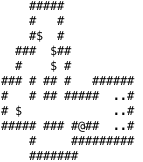
\includegraphics{images/niveau_base}%
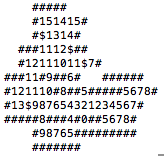
\includegraphics{images/chemin_radar}%
\caption{Plateau rempli par des cases mesurant la distance entre une position donnée}
\end{figure}

Une fois le chemin donnée pour l'intelligence artificielle afin de parvenir au caisse, il faut trouver le chemin le plus porche d'une caisse à une destination. Pour optimiser la recherche il faut garder en mémoire les plateaus deja simulé car il est possible d'obtenir plusieurs fois le même plateau (ce qui évite de potentiel bug de répétition).\\

\subsection{Éditeur de niveau}
Afin d'aller plus loin que ce qui était attendu, nous avons décidé de modéliser un éditeur de niveau. Afin de le rendre le plus efficace possible, nous avons décidé de le rendre totalement indépendant.

L’éditeur de niveau agit au plus bas possible, on interfère directement sur des chaînes. En effet, cela permet d'importer n'importe quel niveau déjà existant ou bien d'en créer un depuis zéro.

Dans l'éditeur, il est possible de :
\begin{itemize}
\item changer case par case les éléments du niveau ;
\item augmenter la taille du niveau en ajoutant directement des lignes ou des colonnes du type de case demandé ;
\item réduire la taille du niveau en supprimant des lignes ou colonnes à un index demandé.
\end{itemize}

L'interface graphique nous permet d’éditer le niveau d'une façon intuitive. Afin de choisir un élément, il suffit de cliquer sur un bouton représentant par une image le type de l'élément désiré. Pour changer une case, il suffit ensuite de cliquer sur celle à modifier. Pour l'ajout ou la suppression de lignes et de colonnes, des boutons sont implémentés afin d'agir rapidement et efficacement sur le niveau. Une fois le niveau réalisé, il peut être sauvegardé, au format \texttt{.xsb}, pour pourvoir le réutiliser plus tard.

\subsection{Interface graphique}

\subsubsection{Lanceur de jeu}

Au lancement du jeu, un lanceur (Figure~\ref{figure:lanceur}) s'affiche afin de guider le joueur dans l'initialisation d'une partie.

\begin{figure}[h!]
\centering
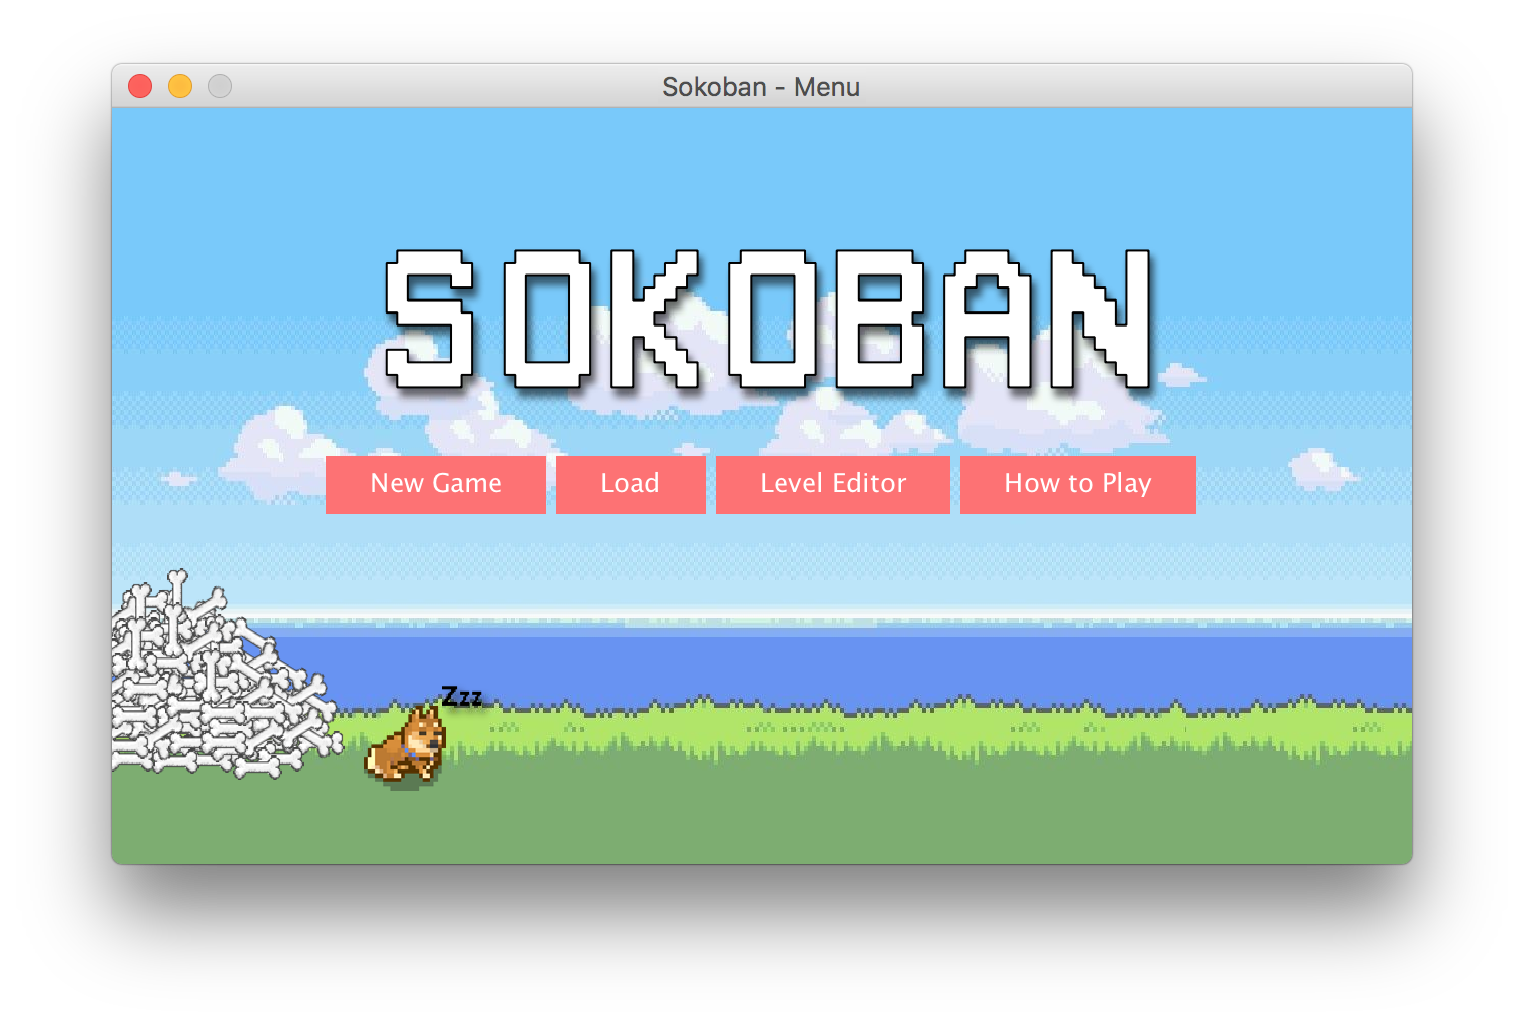
\includegraphics[width=\textwidth]{images/launcher.png}%
\caption{Le lanceur du jeu}
\label{figure:lanceur}
\end{figure}

Il est donc possible de lancer un nouveau jeu seul ou contre l'intelligence artificielle, de charger une partie ou un niveau, d'éditer un niveau soi-même (Figure~\ref{figure:editor}) ou encore de voir les règles du jeu (Figure~\ref{figure:rules}).

\begin{figure}[h!]
\centering
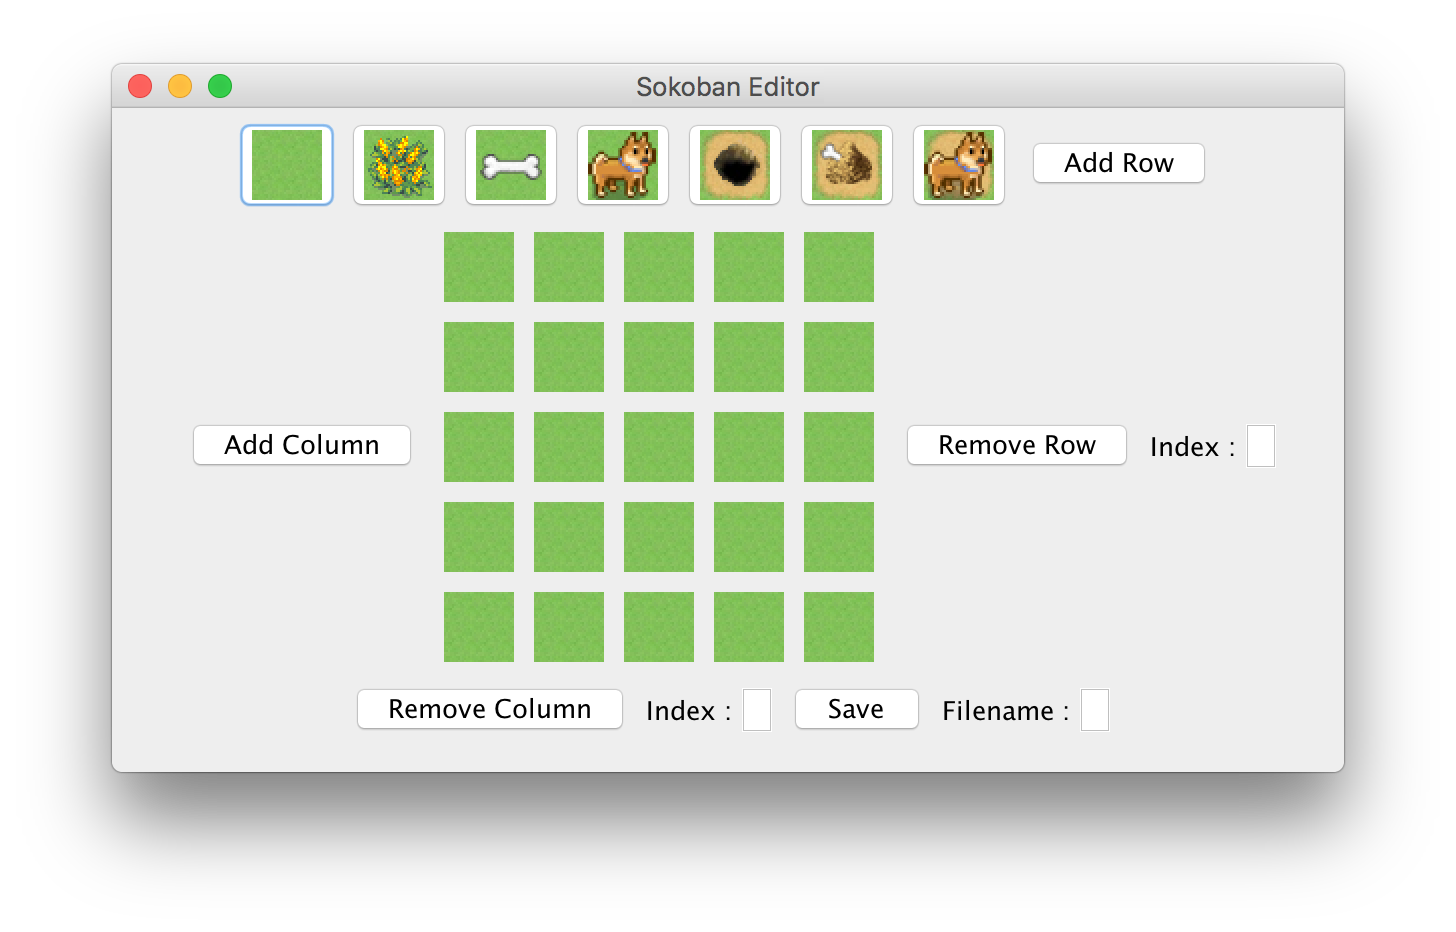
\includegraphics[width=\textwidth]{images/editor.png}%
\caption{L'éditeur de niveau}
\label{figure:editor}
\end{figure}

\begin{figure}[h!]
\centering
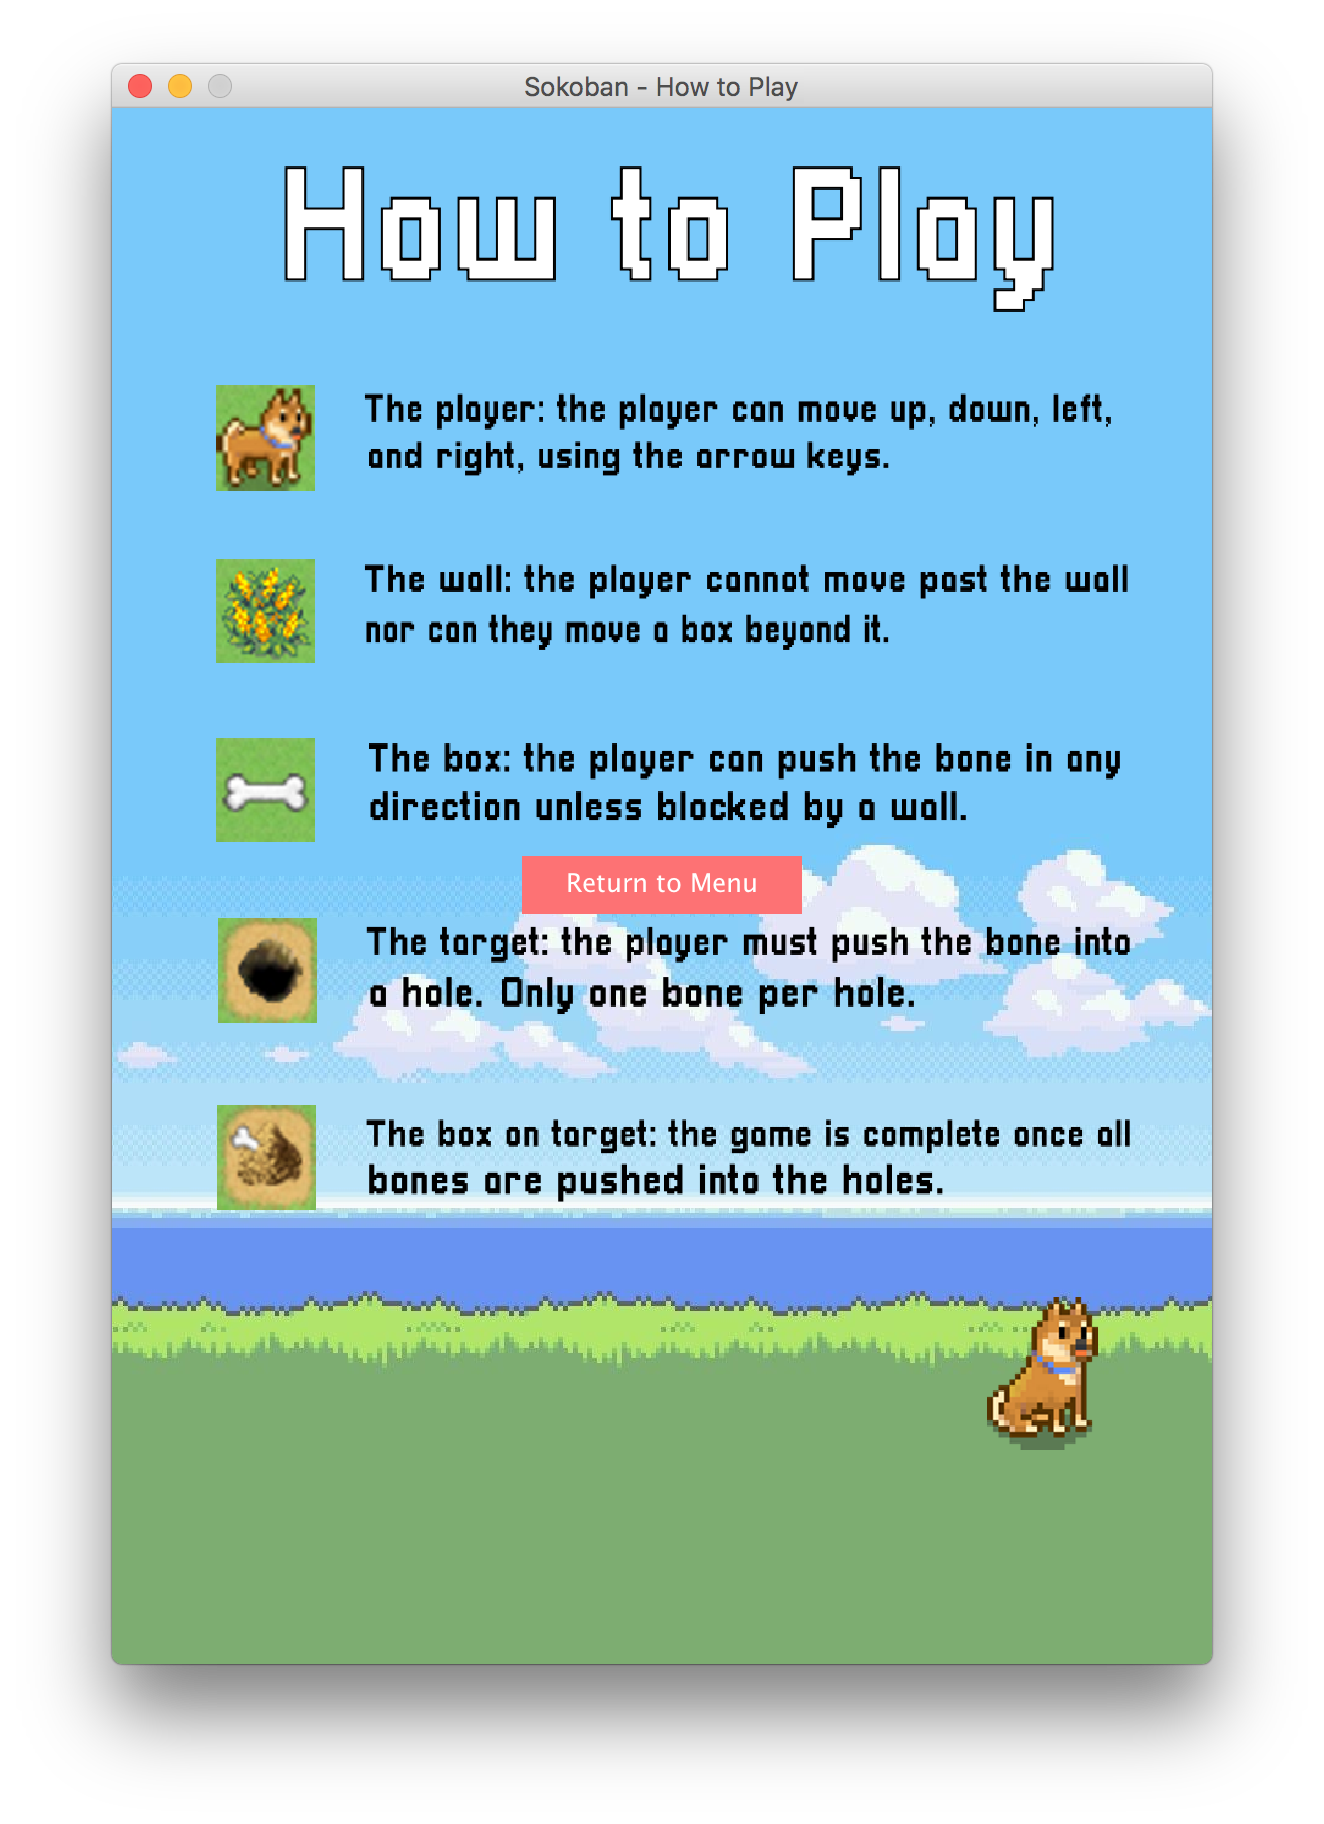
\includegraphics[width=.6\textwidth]{images/rules.png}%
\caption{La fenêtre des règles du jeu}
\label{figure:rules}
\end{figure}


\newpage

\section{Organisation du projet}

Pour réaliser le projet nous avons réparti le travail en plusieurs parties. Deux élèves ont travaillé à temps plein sur l'interface graphique, les deux autres sur la réalisation du jeu de base. Une fois cette phase terminé, nous avons avancé avec tous les membres du projet sur l'intelligence artificielle. Lors de la finalisation de cette phase nous avons réfléchi à l'évolution du projet, grâce à l'implémentation d'options améliorant la qualité du jeu ou de l'intelligence artificielle.

\chapter{Éléments techniques}

\section{Algorithmes}

\subsection{L'algorithme A*}

\label{A*}

L'algorithme A* \cite{wiki:Astar} est un algorithme de recherche de chemin dans un graphe entre un n\oe ud initial et un n\oe ud final. Il utilise une évaluation heuristique sur chaque n\oe ud pour estimer le meilleur chemin y passant, et visite ensuite les n\oe uds par ordre de cette évaluation heuristique. C'est un algorithme simple, ne nécessitant pas de prétraitement, et ne consommant que peu de mémoire.

\subsection{Jeu Bloqué et Deadlock}

\label{deadlock}

Il existe plusieurs façons d'obtenir un jeu bloqué, le plus courant est lorsqu'une caisse est poussée sur une case \emph{deadlock} mais il existe aussi le cas des tunnels, des diagonales. Le cas le plus compliqué à détecter est celui des bipartites.\\

Une case \emph{deadlock} est une case interdite aux caisses, en effet, si une caisse est poussée sur une case \emph{deadlock}, le jeu sera forcément bloqué et aucune résolution du niveau ne sera possible.\\

Une case bloquée est une case où l'un des axes horizontal ou vertical est bloqué. Le jeu n'est pas automatiquement bloqué car si une destination se situe sur un axe non bloqué d'une case bloquée, alors le jeu n'est pas bloqué car une caisse pourrait être poussée à cette destination.\\

\label{gele}
Une case gelée est une case où les deux axes sont bloqués.\\

Positionner  une caisse sur une case gelée entrainera un jeu bloqué.\\

Un tunnel peut-être composé de mur ou de boite. Un tunnel peut devenir une impasse si au bout de celui-ci se trouve un mur ou une caisse.\\

Les blocages de diagonales fermé dans le cas le plus fréquents apparait lorsque 3 caisses sont positionné à coté de façon a former un "L". On appelle cette formation dans les thermes du Sokoban une diagonale, pour que cette diagonale soit fermé il suffit que la derniere case du carré ne soit pas acessible dans ce cas on dit que c'est une diagonale fermé.\\

On peut dire que chaque caisse possedent une position d'arriver, dans certain cas échanger de destination certaines caisse ne posera pas de probleme, sauf une caisse possède qu'une seule possibilité de destination alors le jeu se trouve bloqué par le type de deadlock \og bipartite \fg{}. Pour éviter ce genre de problème il faut connaitre les destinations possibles pour chaque caisse, et vérifier que chaque caisse possède bien au moins une destination, si ce n'est pas le cas alors c'est un blocage bipartite.\\

Les caisses peuvent rendre certaines zone bloqué voir même gelée, il existe certaine cas qui lorsqu'on dépose un caisse sur une destination celle-ci gêle les cases voisines ce qui peut bloquer encore une fois le jeu. \\

Remarque : Chaques coups doivent être calculé à l'avance en effet déposer une caisse peut s'avéré être un piège (entre les blocages de diagonale, celui des case gelêe), il est préférable de bien s'assurer que chaque coups ne créer une situation de blocage.\\

\label{corral}
Le corral est une zone que le joueur ne peut pas atteindre.\\

\section{Structures de données}

Pour représenter les données du jeu, nous avons utilisé un tableau de cases possédant chacune un type (case vide, mur, caisse, joueur, cible, caisse sur cible, joueur sur cible).

\chapter{Architecture du projet}

\section{Diagramme de classes}

\begin{figure}[h!]
\centering
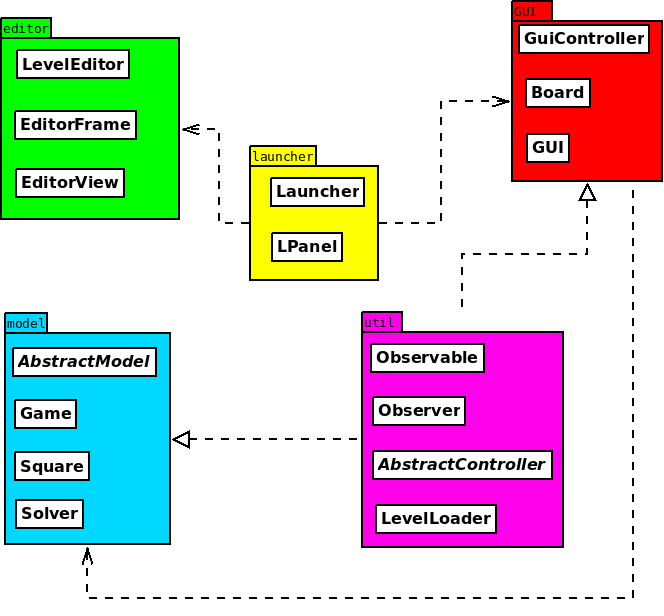
\includegraphics[width=.8\textwidth]{uml/general_uml.png}%
\caption{Principaux packages du projet}
\label{uml:packages}
\end{figure}

\begin{figure}[h!]
\centering
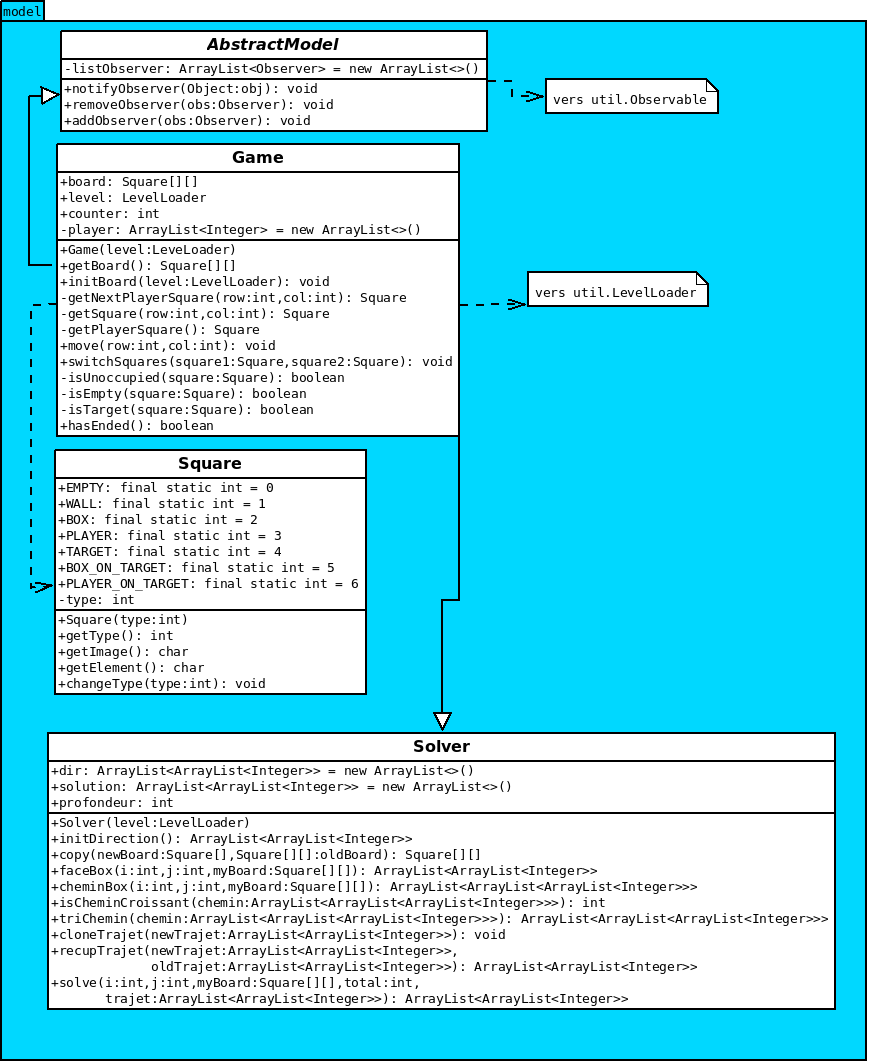
\includegraphics[width=.8\textwidth]{uml/model_uml.png}%
\caption{Diagramme de classes du package \texttt{model}}
\label{uml:model}
\end{figure}

\begin{figure}[h!]
\centering
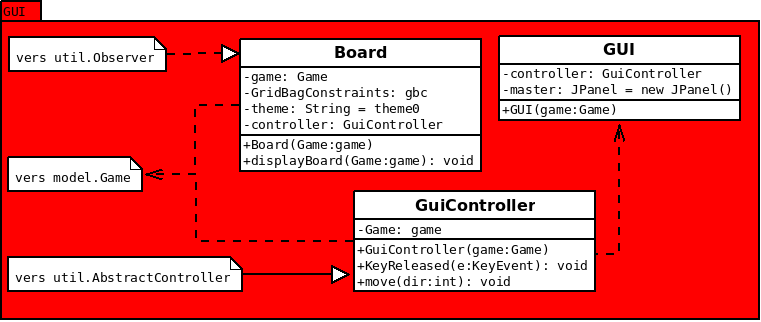
\includegraphics[width=.8\textwidth]{uml/gui_uml.png}%
\caption{Diagramme de classes du package \texttt{gui} (graphical user interface)}
\label{uml:gui}
\end{figure}

\begin{figure}[h!]
\centering
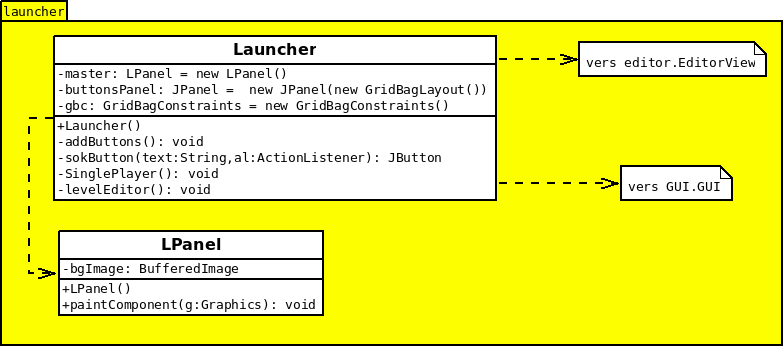
\includegraphics[width=.8\textwidth]{uml/launcher_uml.png}%
\caption{Diagramme de classes du package \texttt{launcher} (lanceur du jeu)}
\label{uml:launcher}
\end{figure}

\begin{figure}[h!]
\centering
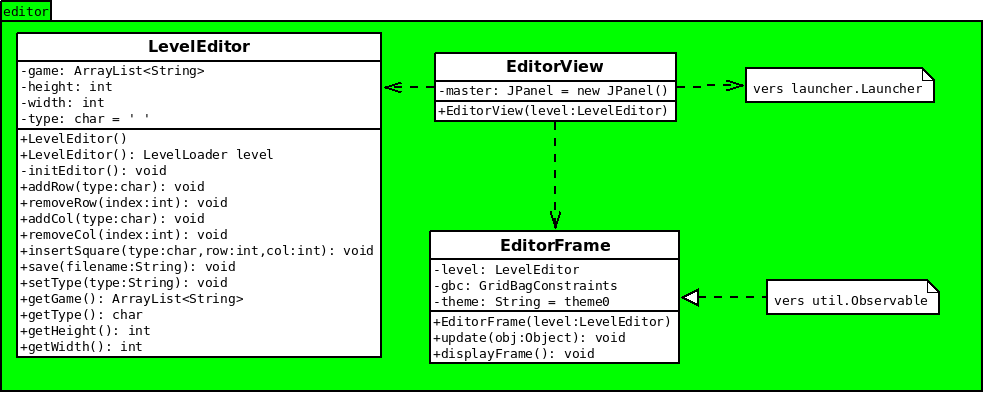
\includegraphics[width=.8\textwidth]{uml/levelEditor_uml.png}%
\caption{Diagramme de classes du package \texttt{editor} (éditeur de niveau)}
\label{uml:editor}
\end{figure}

\begin{figure}[h!]
\centering
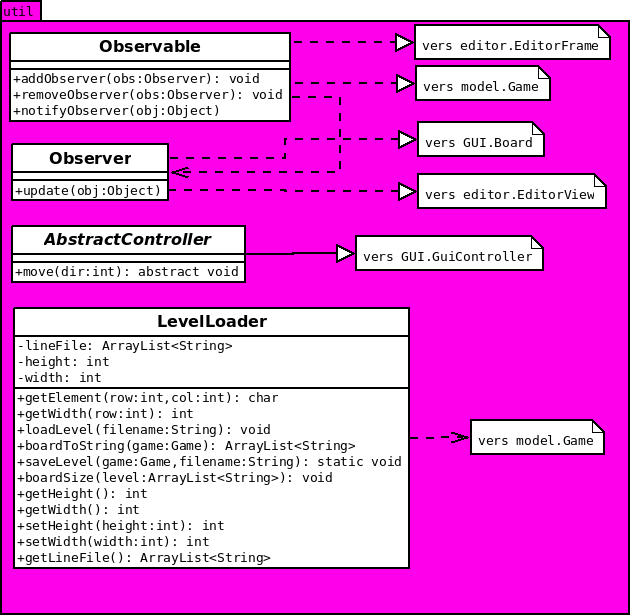
\includegraphics[width=.8\textwidth]{uml/util_uml.png}%
\caption{Diagramme de classes du package \texttt{util} (utilitaires au MVC)}
\label{uml:util_uml}
\end{figure}

\chapter{Conclusion}

\section{Récapitulatif des fonctionnalités principales}

Un plateau permettant de jouer au jeu Sokoban avec toutes les règles, les fonctions de déplacement et d'initialisation lui permet de proposer au joueur une version du jeu jouable sous console.

Une intelligence artificielle permettant de résoudre des niveaux de Sokoban. Elle utilise des fonctions qui lui permettent de se repérer sur le plateau mais aussi des fonctions qui permettent de limiter les coups inutiles grâce à la détection de \emph{deadlock}.

\section{Propositions d'améliorations}

Une seconde version du jeu a été modélisée mais, par manque de temps, nous n'avons pas pu intégrer cette version avec l'intelligence artificielle. Pour l'intelligence artificielle, une amélioration de recherche entre les caisses et les destinations permettraient de résoudre le bug de cycle. L'ajout d'un niveau en coopération pourrait rendre le jeu plus riche grâce a des niveaux dynamiques, ce qui permettrait d'avoir la possibilité de jouer sur le même plateau avec 2 curseurs.

\bibliographystyle{plain}
\bibliography{bibliography}

\end{document}
